\documentclass[tikz,border=2pt]{standalone}
\usepackage{amsmath,amssymb}
\usepackage{pgfplots}
\pgfplotsset{compat=1.18}

\begin{document}
% U(1,4): a flat density of height 1/(b-a) = 1/3 on [1,4]; probabilities are proportional to
% interval length, e.g. P(2 <= X <= 3) = 1/3.
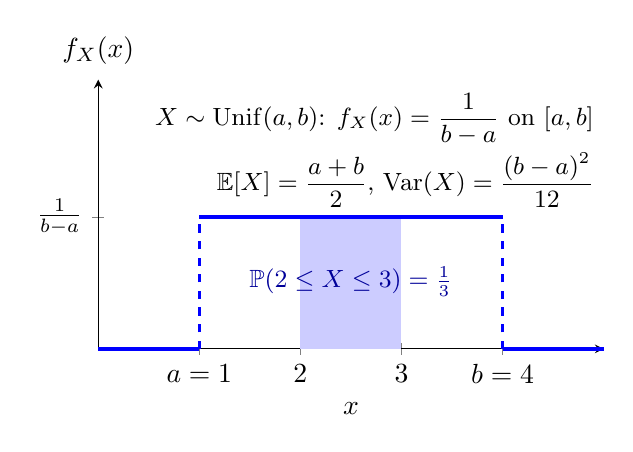
\begin{tikzpicture}
	\begin{axis}[
		axis lines=left, xmin=0, xmax=5, ymin=0, ymax=0.68,
		xtick={1,2,3,4}, xticklabels={$a=1$,$2$,$3$,$b=4$}, ytick={0.3333}, yticklabels={$\tfrac1{b-a}$},
		xlabel={$x$}, ylabel={$f_X(x)$}, ylabel style={rotate=-90, anchor=south, at={(axis description cs:0,1.02)}},
		width=8cm, height=5cm, clip=false
		]
		\fill[blue!20] (axis cs:2,0) rectangle (axis cs:3,0.3333);
		\draw[blue, very thick] (axis cs:1,0.3333) -- (axis cs:4,0.3333);
		\draw[blue, very thick, dashed] (axis cs:1,0) -- (axis cs:1,0.3333);
		\draw[blue, very thick, dashed] (axis cs:4,0) -- (axis cs:4,0.3333);
		\draw[blue, very thick] (axis cs:0,0) -- (axis cs:1,0);
		\draw[blue, very thick] (axis cs:4,0) -- (axis cs:5,0);
		\node[blue!60!black, font=\small] at (axis cs:2.5,0.17) {$\mathbb{P}(2\le X\le3)=\tfrac13$};
		\node[anchor=north east, font=\small, align=right] at (axis cs:5,0.67) {$X\sim \operatorname{Unif}(a,b)$: $f_X(x)=\dfrac1{b-a}$ on $[a,b]$\\[2pt] $\mathbb{E}[X]=\dfrac{a+b}2$, $\operatorname{Var}(X)=\dfrac{(b-a)^2}{12}$};
	\end{axis}
\end{tikzpicture}
\end{document}
